\clearpage
\section{Anhang}
\label{sec:appendix}

Im Anhang werden Vorgehen in den verschiedenen Abschnitten näher erläutert. Es werden alle Hintergrundinformationen, die nicht direkt für die Arbeit selbst relevant sind gesammelt und dargestellt.

\subsection{Vorgehen bei der Untersuchung der Curricula}
Um auszuarbeiten, wie die aktuelle Situation an deutschen Hochschulen und Universitäten ist, wurde der Hochschulkompass der Hochschulrektorenkonferenz verwendet \cite{hochschulkompass}.
Auf der Webseite wurden Studiengänge der Informatik gesucht, und nach folgenden Kriterien mithilfe der Filterfunktion der Webseite sortiert:

\begin{itemize}
    \item Abschluss Bachelor/Bakkalaureus (Da Programmieranfänger betrachtet werden sollen, macht es im Kontext keinen Sinn, weiterführende Studiengänge oder Masterprogramme zu berücksichtigen)
    \item Studientyp Grundständig (Siehe Abschluss Bachelor/Bakkalaureus)
    \item Fachsuche Informatik (Speziellere Studiengänge wie Bioinformatik und Wirtschaftsinformatik wurden ausgeschlossen, um Überschneidungen an den Schulen zu meiden. Es wurde immer ein Studiengang pro Institution untersucht, der sich möglichst nah an der Allgemeinen Informatik kategorisieren lässt)
    \item Studienfeld Angewandte Informatik oder Informatik (Siehe Fachsuche)
    \item Studienformen Vollzeitstudium (Ein weiteres Kriterium, um Überschneidungen zu meiden und die Studiengänge weiter auszusortieren)
    \item ohne Lehramt (Wurde in den Filtern aussortiert, da die Lerninhalte sowohl Informatik als auch Erziehungswissenschaften umfasst, und somit nicht im Fokus der Arbeit liegen)
\end{itemize}

Nach der Anwendung der Filter wurden noch insgesamt 425 Treffer angezeigt, die erst im späterem Verlauf der Arbeit weiter reduziert wurden (siehe \nameref{sec:sorting}).

\subsubsection{Zeit Management}\label{sec:time_management}
Aufgrund dessen, dass die Curricula Analyse nicht der Schwerpunkt der Bachelorarbeit sein sollte, musste abgewägt werden, wie viel Zeit in das Thema investiert werden soll.
Hierbei wurden mehrere Risiken gesehen. Zum einem ist es möglich, dass man durch Internetrecherche alleine nicht erschließen kann, welche Inhalte ein Modul hat.
Zum anderen ist, das größere Risiko wahrscheinlich, der Zeitfaktor. Es ist ungewiss, wie lange es dauert, jedes Modul zu untersuchen, da jede Institution ihre Informationen anders sortiert, bereitsstellt und handhabt.

Um die Zeit in einem realistischen Rahmen zu halten, wurde in Erwägung gezogen, einen Zeitraum festzulegen, in dem so viele Studiengänge wie möglich betrachtet werden, und diese anschließend die Forschungsmenge darstellen. Dieser Zeitraum könnte etwa auf 2 Arbeitstage fallen. Auch abgewägt wurde, die Studiengänge nach Anzahle der Studierenden zu sortieren, und die 50 am meisten besuchtesten Insititutionen zu betrachten.

Es wurde allerdings ebenfalls notiert, dass das ungewisseste Kriterium hier die Zeit war, die benötigt wird, um einen Studiengang zu untersuchen. Möglicherweise müssen die Methoden zur Reduktion der Zeit gar nicht angewandt werden, wenn sich die Risiken nicht erfüllen. Zunächst wurde daher versucht, abzuwägen, wie lange die Dauer der Analyse prinzipiell grob einzuschätzen war.
In einer isolierten Probe wurden fünf zufällige Universitäten betrachtet (In diesem Fall die ersten fünf Suchergebnisse des Hochschulkompasses, die HS Furtwangen, die Ruhruniversität Bochum, die Hochschule Fulda, die Friedrich-Schiller-Universität Jena, und die Hochschule Konstanz).
Hierbei dauerte es etwa 10 Minuten, um entsprechende Informationen über alle 5 Studiengänge zu erlangen.
Bei den 121 verbleibenden Informatik Studiengängen wurde die Zeitdauer also grob auf 4 Stunden eingeschätzt, ein realistischer Zeitraum zur Sammlung der Daten. Mit diesen neuen Informationen wurden die Methoden zur Zeitreduktion wieder verworfen.

Letztendlich wurde für die Analyse doch ein ganzer Arbeitstag benötigt, aber die reduzierte Menge der Studiengänge durch die Filter war bereits genügend, um die Daten in einem angemessenem Zeitraum zu sammeln.

\subsubsection{Untersuchung der Daten}\label{sec:sorting}
Bei der Analyse der Curricula wurde systematisch vorgegangen. Mithilfe eines Webscrapers wurden alle nötigen Informationen als JSON extrahiert, und in einer Excel Tabelle sortiert.
Es wurde festgestellt, dass die Filterfunktion des Hochschulkompasses nicht ausreichend war, um die Datenmenge zu reduzieren. Die Studiengänge wurden daher noch einmal manuell aussortiert, nach weiteren Kriterien.

\begin{itemize}
    \item Kein Allgemeiner Informatikstudiengang (z.B Bioinformatik oder Wirtschaftsinformatik)
    \item Zweitfach oder Nebenfach Informatik
    \item Teilzeitstudium
    \item Mehrere Studienorte für einen Studiengang (Hierbei sind die angebotenen Module teils nicht eindeutig zuordbar)
    \item Doppelte Studiengänge für eine Institution (Etwa wenn sowohl Angewandte, als auch Allgemeine Informatik angeboten wird. Hierbei wurde sich immer für den Allgemeineren Studiengang entschieden. Zwischen internationalen und deutschen Studiengängen wurde immer der deutsche Studiengang gewählt)
\end{itemize}

Für die meisten Studiengänge ließen sich die nötigen Informationen in sehr kurzen Zeiträumen mit einer Suche nach dem Studienverlaufsplan, sowie dem Modulhandbuch für die Informatik finden.
Hierbei wurde der Studienverlaufsplan genutzt, um herauszufinden, welcher Kurs als Einführung in die Programmierung im ersten Semester dient, und das Modulhandbuch, um zu extrahieren welche Programmierparadigmen und Sprachen im Kurs verwendet werden.

Nicht alle Module listeten die benötigten Informationen. Es wird in der Analyse grundsätzlich unterschieden zwischen zwei Fällen. Zum einem, Studiengänge, die zwar ein Modulhandbuch zur Verfügung stellten, dieses aber nicht explizit spezifiziert welche Paradigmen und Spachen verwendet werden (Markiert als "Unspezifisch"). Zum Anderem gibt es noch den Fall, dass kein Modulhandbuch öffentlich zur Verfügung steht. Dies kann etwa der Fall sein, wenn die Insititution Informationen nur auf Anfrage herausgibt, oder das Modulhandbuch einfach nicht aufzufinden war. Es wurde davon abgesehen, die Insititutionen zu kontaktieren, um einen neuen ungewissen Zeitfaktor zu vermeiden. Die Studiengänge ohne Modulhandbuch wurden leer gelassen, und sind in der Excel rot markiert. In der Grafik zu darstellung der Ergebnisse sind diese Datensätze in "Keine Infos" kategorisiert.

Die Excel Tabelle mit den extrahierten Daten lässt sich im Repository der Bachelorarbeit finden \cite{repoxlsx}.

\subsection{Auswahl des Problemes im Praxisteil}
Die Auswahl des Programmierproblems in Abschnitt 4 der Arbeit erfolgte an mehreren Kriterien. Zum einem sollte ein relativ einfaches Problem gewählt werden, welches weniger zu innovativer Lösungsfindung anregen sollte, als mehr nur zur Demonstration eines Zweckes dienen sollte.
Zunächst wurde sich hierbei entschieden, einen Algorithmus zur automatischen Lösung und Erstellung eines Sudoku zu schreiben.
Bei einem Sudoku handelt es sich um ein klassisches Rätsel, bei dem auf einem 9x9 großem Feld in jeder Zeile, Spalte, und in jeder 3x3 großen Box jede Zahl von 1 bis 9 nur ein mal vorkommen darf.

Das Problem eignete sich zum Untersuchen und Lernen von funktionaler Programmierung, da alle wichtigsten Aspekte von funktionaler Programmierung benötigt wurden, um das Problem im Paradigma erfolgreich umzusetzen (Rekursion, Funktionen Höherer Ordnung, Komposition, Unveränderlichkeit). Es wurden ebenfalls alle CT Aspekte ausreichend abgedeckt.

\begin{description}
    \item[Dekomposition] Herunterbrechen in Teilprobleme. Beispielsweise, Validierung des Sudoku, dann Untersuchen der Spalten, Zeilen und Boxen separat.
    \item[Abstraktion] Rätsel in Datenstrukturen umwandeln. Beispielsweise, Überlegunge, wie das Brett und die Felder am Besten im Code abgebildet werden können.
    \item[Algorithmen] Zur Implementierung des Solvers.
    \item[Debugging] Wie kann das Sudoku effizient gelöst werden? Evaluierung der Lösung, und Erkennen von Fehlerpotential in den einzelnen Unterfunktionen.
\end{description}

Letztendlich wurde sich allerdings doch für ein anderes Problem entschieden, da Sorgen hinsichtlich der Umsetzbarkeit im gegebenen Zeitrahmen bestanden.
Es wurde sich letztendlich für die Türme von Hanoi entschieden, aufgrund einer Empfehlung des betreuuenden Prüfers, sowie das Vorkommen der Aufgabe im ersten Aufgebenblatt des verwendeten Kurses, um Haskell zu lernen. % TODO Wow Umformulierung bitte
Das Problem vetritt ebenfalls wichtige Aspekte von FP, vor allem das Konzept des Backtrackings. Auch die CT Aspekte waren wiederum erkennbar vetreten, was letztendlich zur Entscheidung führte.

\begin{description}
    \item[Dekomposition] Überlegung welche Teilprobleme es gibt. Ein bisschen weniger offensichtlich als beim Sudoku Solver, aber beispielsweise die Validierung der Züge und die tatsächliche Durchführung sind zwei verschiedene Verantwortungen.
    \item[Abstraktion] Überlegung, wie die Pins und Holzplatten abgebildet werden können. Wie wird deutlich, welche Platte zu welchem Pin gehört? Wie wird die Größe der Platten deutlich? Hierbei können beispielsweise Integer verwendet werden.
    \item[Algorithmen] Zur tatsächlichen Implementierung des Problems.
    \item[Debugging] Ebenso wie der Sudoku Solver gibt es hier mehrere Lösungen, die abgewägt werden können.
\end{description}

\subsection{Vorgehen im Praxisteil}
Der Autor hatte vor der Bachelorarbeit keine großen Vorkenntnisse in FP, und keine Erfahrungen mit Haskell. Um die Sprache zu lernen, wurde den offiziellen Empfehlungen der Haskell Dokumentation gefolgt. Hierbei war das sogenannte REPL (read-eval-print-loop) besonders hilfreich. Die interaktive Programmierumgebung nimmt einzelne Nutzerinputs, evaluiert diese und gibt den Output an den Nutzer zurück. Im Kontext der CIS 194 Vorlesung wurde das REPL ebenfalls zur Einführung in Haskell Variablen verwendet.
Anfänger können so schnell und barrierelos mit der Syntax und den Ausdrücken in Haskell experimentieren, und so praktische erste Programmiererfahrungen machen.

\begin{figure}[H]
    \centering
    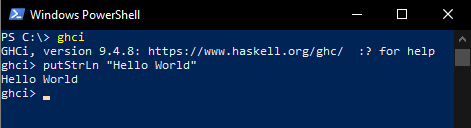
\includegraphics[width=1\linewidth]{Figures/Anhang/ghci}
    \caption{Verwendung von GHCi in der Windows Powershell}
\end{figure}

Um Haskell Syntax und gerenelle Prinzipien zu lernen, wurden zunächst die ersten Aufgaben der CIS 194 Hausaufgaben bearbeitet.